% --- Configuration ------------------------------------------------------
% add shortcut for github url of this chapter
\def \GITHUB {\GITHUBBASE/01_introduction}

% --- Document -----------------------------------------------------------
\chapter{Introduction}
\label{cha:introduction}
%
\firstthought{Listening} to music plays an important role in the social and
cultural life of human beings.
Musical instruments found in archaeological excavations can be dated back as far
as 40\,000 years in the past.\autocite[For an overview see][]{dErrico2003}
There is a variety of different types of music and the time spent for
listening to music is still increasing. One of the preconditions for this
increase was the invention of the first electroacoustical transducer -- the
telephone in 1876. After that it was possible to listen to music without the
presence of a musician.
The digitalisation and vast availability of music in the last years made it
even easier to listen to music.\autocite{Sloboda2009}

Due to the importance of communication and music in our everyday life, the
electroacoustical presentation of sound has advanced quickly after the invention of
the telephone.
It was noted that when all sound was presented only by a single transducer the
spatial impression of a recorded sound -- e.g. an orchestra -- is lost.
It would enhance the listening experience if the spatial impression of the
sound could be recreated during the presentation. This inspired Steinberg and
Snow\autocite{Steinberg1934} to their idea of recreating a whole sound field in
the audience area. But they noted already that they would basically need an
infinite number of receivers and transmitters to do this.
In an experiment they arranged a setup consisting of only two microphones and
two loudspeakers and showed that this low number of loudspeakers ``give(s) good
auditory perspective''.

The ideas and results from Steinberg's and Snow's paper are still part of the main research
topics in spatial audio. What is the best way to give a good spatial
impression of the presented sound? How many loudspeakers are needed to do this?
Is it possible to create a spatial
extended sound field in a convincing way? What is the influence of the spatial impression on
the overall quality a listener experiences while listening to the played back
sound?

The goal of this thesis is to investigate these questions with a focus on
\ac{SFS} techniques and their perception. The main question targets the analysis
of which parts of an imperfectly reproduced sound field are perceived as
imperfect
by the listener and which parts are not.
As the work in the field of audio coding has demonstrated, the listener
may be insensitive to a large amount of ``errors'' in a sound signal.
In addition, a link to the underlying
technical parameters that cause the imperfection of the sound field will be
established in order to control the amount of errors in a systematic way.
This work is a foundation for the investigation of the larger question of
how these systems influence the quality experienced by the listener.

\newthought{For a more detailed} understanding of the research questions the basic
principles of the auditory system that contribute to the perception of a spatial
sound scene are discussed in this introduction chapter. In addition, a short
overview of different spatial sound reproduction techniques is provided,
followed by a theoretical framework to establish how to talk about quality of spatial
audio and how to investigate it.

In the second chapter the mathematical framework of the different methods for
creating a spatial extended sound field is presented and the formulas for
the calculations of loudspeaker signals are provided. The methods are restricted to
analytical solutions of the integral equation that describes the sound field
synthesis problem -- namely \ac{WFS} and \ac{NFC-HOA}. The presentation of the
framework is motivated by the idea of highlighting that both methods have the
same foundation and are comparable in several ways.\autocite[This idea is
developed in more detail in][]{Ahrens2012}
This deviates from classical
research papers in the field of \ac{WFS} and \ac{NFC-HOA} that employ
different mathematical frameworks due to their historical independence.

The limitations of today's hardware in practical implementations
-- distance between and number of
loudspeakers -- lead to several deviations in the created sound field from the
desired one. The possible implications of these deviations and connections to
the underlying hardware and mathematical parameters are discussed in
Chapter\,\ref{cha:sound_field_errors_and_their_perceptual_relevance}.
Considering the functioning of the human auditory system,
hypotheses are formulated about the influences of the deviations on their
auditory perception.
The hypotheses point directly to the research questions that will be dealt with
in different psychoacoustic experiments as presented in
Chapter\,\ref{cha:psychoacoustics}.

Before that, Chapter\,\ref{cha:binaural} discusses the method applied for the
psychoacoustic experiments.
The challenge of psychoacoustic experiments for spatial audio is
the dependence of the results on the position of the listener. It is not only of
interest how the perception is at a particular point, but how it is
in the whole listening area. Another challenge is to systematically investigate
the influence of the technical parameters of the underlying presentation
methods on perception. For sound field synthesis methods the number of and distance
between the loudspeakers are especially critical parameters and should be adjustable in a
wide range from two up to several thousand loudspeakers.
Simulating all systems with binaural synthesis is a solution to these problems.
The approach can evoke errors, however,  and a large part of the fourth chapter
investigates if binaural synthesis is suitable as a tool for answering the psychoacoustic
research questions.

After assessing the influence of the technical parameters on the perception for some
setups it is of interest to predict the perception of the listener to
investigate every possible setup. Chapter\,\ref{cha:modelling} shows this
for the case of localization for \ac{WFS} and
\ac{NFC-HOA}. A binaural auditory model is fed with the signals reaching the
ears of the listener
and is shown to be able to predict the perceived direction for a
given source in the sound field.

The last chapter summarizes the results and discusses the
implications of the results for further investigations of the quality of spatial
audio systems.



%%%%%%%%%%%%%%%%%%%%%%%%%%%%%%%%%%%%%%%%%%%%%%%%%%%%%%%%%%%%%%%%%%%%%%%%%%%%%%%%
\section{The Human Auditory System}
\label{sec:hearing_of_the_human_auditory_system}
%
For human beings hearing means that sound signals arriving
at the eardrums of both ears are processed by different mechanisms to finally
lead to a corresponding perception -- as illustrated by
Figure\,\ref{fig:auditory_scene}.
%
\begin{figure}
    \centering
    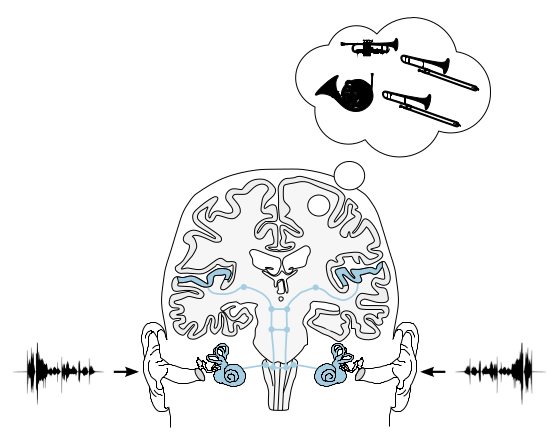
\includegraphics[width=.8\columnwidth]{fig1_01/fig1_01}
    \caption{The human auditory system. The two ear signals are processed by the
    outer, middle, and inner ear. In the inner ear they are transformed into
    neuronal signals which are then analyzed at different interlinked stations
    in the brain. The interlinking of both ear signals already happens
    at a low level in the brainstem. In the brain itself a representation of
    the external ear signals in the form of an auditory scene is the final stage.
    This figure is based on~\cite{Grothe2010,Talbot2011a,Chittka2005}.
        \reproduce{\GITHUB/fig1_01}
    }
    \label{fig:auditory_scene}
\end{figure}

In the discussion of correspondences
between physical sound objects and the corresponding perceptional
objects the following terms are used. As long as the physical
sound signals outside of the listener are considered, the terms
\emph{sound event(s)} and \emph{sound scene(s)} describe what is presented to
the listener. A sound event corresponds to the signal emitted by
a physical sound source such as a
human speaker or a loudspeaker. A sound scene is a composition of different
sound events.
The number of sound events originally involved in the creation of these
signals cannot be estimated for all situations, if only the two signals arriving
at the ears of the listener are considered.
This fact
is utilized by sound field synthesis techniques: to generate the sound field
corresponding to a single sound event with the help of a very large number of
individual sound
events.\sidenote[][-1cm]{\cite[This is better known as the Huygens-Fresnel principle,
see e.g.][]{Huygens1912}}

The superposed signals are transformed into a movement of the
eardrums, transformed into neural activity in the inner ear and further interpreted by
the brain. The final perceptual output is a complex \emph{auditory scene}
composed of single \emph{auditory events}. Listeners can distinguish 
single auditory events and steer their auditory attention to one of the events.
Furthermore, they are associated with different perceptual attributes such as
loudness, pitch, duration, timbre, and spatial features.\autocite{Letowski1989}
Together, the different features form the aural character of an auditory event
or scene.

As such, the process of hearing generates an auditory scene
from the presented sound scene. The extraction of
single auditory events from the eardrum signals is referred to as
auditory scene analysis. It is obvious that there is no linear function
that is able to describe the mapping of sound events to auditory events, because
the number of sound and auditory events does not have to match.
For example, imagine the following setup: two loudspeakers are placed in an
anechoic environment and play exactly the same signal to a listener placed
in the middle of the loudspeakers at a distance of a few meters.
In that case, the listener perceives only one auditory event in the center of the two
loudspeakers, a phenomenon applied in stereophony. Assume now that the same equipment
is placed in an echoic room. The room is by itself not a new sound source, but
adds reflective elements to the sound scene. Listener perceive the room as additional
features to the initial auditory event.

Note that an auditory event is on a lower abstraction level
than an \emph{auditory object}
that requires even more processing of the brain -- including multi-modal
processing.\autocite[A discussion of auditory objects is presented in][]{Kubovy2001}
For the topics investigated in this thesis it is
sufficient to limit the considerations to auditory events.

\newthought{After introducing} the terminology for describing auditory
perception, the processing of the sound signals by the auditory system is
discussed in more detail.
In a first step the sound field created by all sound events is filtered by
the outer ears of the listener. Thereby, its frequency content is modified depending on the
incidence direction. This provides a relevant cue
for the perception of the vertical direction of a sound
source.\autocite[See p.\,97ff in][]{Blauert1997}
In the ear canal, all signals from the sound events are superimposed and excite
the eardrums.
The oscillation of the eardrums is amplified by the auditory ossicles in the
middle ear and coupled to the inner ear. At this point the mechanical signal is
dispersed and converted into neuronal signals.
The neuronal signals are able to preserve the temporal information of the sound
signals up to a frequency of about $1.5$\,kHz, for higher frequencies only the
temporal information of the envelope can be extracted. The information on
higher frequencies is not completely lost in this process because the
dispersion of the mechanical signal in the inner ear distributes the signal energy
regarding its frequency content and performs a frequency-place-transformation
comparable to a Fourier transformation.
The neuronal
signals are transmitted to different places in the brain starting with the
\emph{cochlear nucleus}, the \emph{superior olivary complex}, and the \emph{lateral
lemniscus} in the brainstem
going further to the \emph{inferiror colliculus} in the midbrain and the
\emph{medial geniculate body} in the thalamus before reaching the \emph{primary
auditory cortex}.\sidenote[][-1cm]{\cite[E.g.][]{Grothe2010}}

\begin{figure}[t]
    \centering
    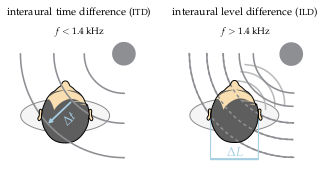
\includegraphics{fig1_02/fig1_02}
    \caption{Interaural differences occur between both ear signals for sources to the
    side of the listener. For low frequencies \acp{ITD} are the dominant cue,
    for high frequencies \acp{ILD} are more reliable.
    The figure is based on~\cite{Grothe2010}.
        \reproduce{\GITHUB/fig1_02}
    }
    \label{fig:itdild}
\end{figure}
%
An interaction between the neuronal signals of both ears appears already
at a very low level, namely the \emph{superior olivary complex}. At this point
differences between the two signals can be analyzed that provide evidence for
the direction of an auditory event in the horizontal plane. This process of
attributing a direction in the horizontal plane to an auditory event is called
\emph{localization} in this thesis. Usually localization also includes
the vertical direction and the distance of the auditory event, but these aspects
are not considered in this work.
The two main differences that allow a calculation of a direction of incidence
are the \acf{ITD} and the \acf{ILD} of the two ear signals as indicated by
Figure\,\ref{fig:itdild}. The \ac{ITD} exploits the fact that the time of arrival
at each ear depends on the direction of the sound. This requires a
high temporal accuracy of the auditory system, which is only provided for
frequencies up to $1.4$\,kHz. The frequency limit corresponds roughly to the
diameter of a human head that is another natural limit for the usage of the \ac{ITD}.
For higher frequencies more than one wave length of the sound waves
lies between the two
ears. Thus the \ac{ITD} becomes an ambiguous cue. For \ac{ILD} it is the opposite.
\ac{ILD} results from the fact that the human head is not transparent for sound
waves and scatters them. That leads to a difference in sound pressure level
depending on the incidence angle of the sound. For frequencies below $1.4$\,kHz
the influence of the head can be neglected, whereas for higher frequencies the level
differences are relevant. Sound components with wave lengths similar to the head diameter are
diffracted around the head and reach the opposite ear.
This has motivated the duplex theory\autocite{Rayleigh1907} of localization,
assuming that the \ac{ITD} cues are used for low frequencies and the
\ac{ILD} cues for high frequencies. How the different cues are combined
to form a directional perception is presented in
Section\,\ref{sec:localization} and \ref{sec:binaural_models}.

\newthought{The goal} of every sound field synthesis technique is
to provide the same spatial cues as in the original sound field, as opposed
to the sweet-spot
phenomenon of stereophony that is explained in the next section. In order to
achieve this, highly correlated signals are presented to
different loudspeakers. This scenario is roughly equivalent to delaying and
summing up the same signal. Thereby a comp-filter like amplitude spectrum
appears that can introduce severe timbral changes.
Besides, it is possible that the creation of completely unnatural
signals with \ac{SFS} lead to the perception of
additional spectro-temporal artifacts.

This thesis concentrates on a subset of attributes of auditory events that are
relevant for assessing sound field synthesis methods, namely timbre, direction,
and technical artifacts. The different attributes will be discussed in detail in
Chapter\,\ref{cha:psychoacoustics}, which investigates also the influence of
several physical parameters of \ac{SFS} on those attributes.

In the next section, a short overview of different spatial sound presentation
techniques, including stereophony and \ac{SFS} is presented.


%%%%%%%%%%%%%%%%%%%%%%%%%%%%%%%%%%%%%%%%%%%%%%%%%%%%%%%%%%%%%%%%%%%%%%%%%%%%%%%%
\section{Spatial Sound Presentation Techniques}
\label{sec:spatial_sound_reproduction_and_synthesis_techniques}
%
In this thesis spatial sound presentation refers to all methods that try
to recreate some of the spatial aspects of a given sound scene by applying more
than one loudspeaker.
The first ever practical attempt of spatial sound reproduction dates back to
1881, only five years after the invention of the first monaural transducer.
Back then, two parallel telephone channels were used to transmit recorded
music to the homes of the listeners.\autocite{DuMoncel1881a}
The basic idea was the ability to influence the interaural
differences between the two ear signals of the listener. That was achieved by
recording a sound scene with two microphones placed at different positions 
and feeding the recorded signals to the two telephone channels.

Later on the idea advanced to the technique of \emph{binaural presentation} where the basic
principle is to recreate the ear signals at both ears as they would appear in reality.
This can
be achieved by placing two microphones in the ears of the listener for recording and playing the
recorded signals back via headphones afterwards.
Binaural presentation has advanced in the last decades by measuring the
acoustical transmission paths between a source and the ears of a listener, so called
\acp{HRTF}. Afterwards these can be used to create any sound scene as long as
the required \acp{HRTF} are available. Due to the good control of the ear signals
that arrive at the listener's ears this method is very accurate in creating directional
cues and will be applied in this thesis for simulating the ear signals for
different loudspeaker setups.
%
\begin{figure}[t]
    \centering
    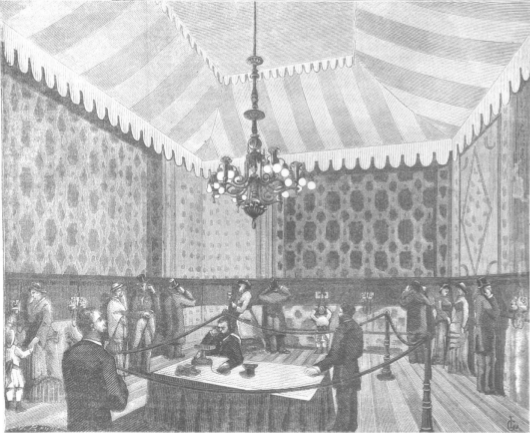
\includegraphics[width=.8\columnwidth]{fig1_03/fig1_03}
    \caption{Setup of stereophonic telephones at the exhibition 1881 in
    Paris. Figure from \cite{DuMoncel1881a}
        \reproduce{\GITHUB/fig1_03}
    }
    \label{fig:stereo_telephone}
\end{figure}

Spatial sound presentation via loudspeakers started in the 1930s, the time when
Blumlein invented the stereophonic recording and
reproduction\sidenote[][]{\cite{Blumlein1958}} and Steinberg and Snow discussed the idea of
the acoustical curtain.\autocite{Steinberg1934}
The original idea of the latter was to create a sound field that mimics the real sound
scene. Their practical implementation with two or three loudspeakers was not able
to achieve this. With such low numbers of loudspeakers the sound field is only
controllable at single points in space. This corresponds to the classical
stereophonic setup consisting of a fixed listener position between the two
loudspeakers at a distance of around $2$\,m.
The human head has a diameter of around $20$\,cm and hence only one ear can
be placed at the point where the sound field is as desired. But as Steinberg and
Snow discovered for their acoustic curtain, the spatial perception of the
listener is not disturbed as long as she does not move too far away from a line
on which every point has the same distance to both loudspeakers.
By staying on that line the listener perceives an
auditory event in the center of both loudspeakers, if the same acoustical signal
is played through them. If the amplitude of one of the loudspeakers is changed
the auditory event is moved between the two speakers. The connection of the
amplitude difference between the loudspeakers and the actual position of the
auditory event is empirical and is described by so called panning
laws.\sidenote[][]{\cite{Leakey1959}}
If the listener leaves the central line, the position of the auditory event
will always be located at the position of one of the two loudspeakers. The area in which the
spatial perception of the auditory scene works without considerable impairments
is called the \emph{sweet-spot} of a given loudspeaker setup. It is indicated
by the blue color in Figure\,\ref{fig:stereophony}.
To explain why the spatial perception of the listener is correct at the
sweet-spot although the sound field is not, the theory of \emph{summing
localization} was introduced by Warncke in 1941.\sidenote[][]{\cite[A discussion is
provided in][p.\,204]{Blauert1997}}

\newthought{In the last years} the stereophonic setup was expanded to 5.0 surround
and even larger setups\sidenote[][]{\cite[E.g.][]{Hamasaki2005}} and the panning laws were
formulated in a more general way dealing with setups using multiple
loudspeakers.\sidenote[][]{\cite{Pulkki1997}}
These approaches could not fix the sweet-spot problem, but added a richer
spatial impression because sound is no longer restricted to come from the front.
%
\begin{figure}[t]
    \centering
    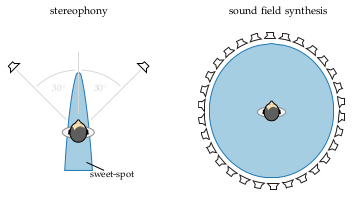
\includegraphics{fig1_04/fig1_04}
    \caption{Loudspeaker setups for two channel stereophony
    and sound field synthesis. The area marked in blue describes the positions were the
    listener can move to and still perceives the same spatial impression. This
    area is smaller for stereophonic setups and is called the
    sweet-spot. The figure of the stereophony setup is a modified version of
    \cite[][Fig.\,1.1]{Ahrens2012}.
    \reproduce{\GITHUB/fig1_04}}
    \label{fig:stereophony}
\end{figure}

Before 5.0 surround there were other approaches to enhance the spatial impression of
stereophony. From the 1970s onwards quadro\-phony and
Ambisonics\autocite{Gerzon1973} were developed in
order to provide a surround experience with four loudspeakers. The basic idea of
Ambisonics is comparable to nowadays \ac{NFC-HOA} for
a larger number of loudspeakers: to describe an extended sound field by spherical
basis functions that can be synthesized by any spherical or circular loudspeaker
setup. In practice, the restriction of the limited number of loudspeakers has led to the usage
of only two spherical basis functions. The results are
loudspeaker signals that are comparable to the case of panning in
stereophony with the difference of more active
loudspeakers.\autocite[E.g.][]{Frank2013}
If more than four loudspeakers and more than two basis functions
are applied the term is changed to \ac{HOA} to highlight this fact.
For the perceptual side of Ambisonics the sweet-spot problem exists as well.
The explanation of this sweet-spot is only partly covered by the
theory of summing localization, because that theory is not well investigated for
several sound sources coming from all directions. This provoked a high number of
different optimizations of the loudspeaker signals by the Ambisonics community.


\newthought{All of the} methods described so far are able to provide a
convincing spatial impression at a specific listener position within the
loudspeaker setup. That means none of them can handle an equally good spatial
impression for a bigger audience.

In the late 1980s the old idea of Steinberg and Snow to reproduce a
complete sound field came to new life due to the fact that now arrangements of
more than 100 loudspeakers became possible.\autocite{Berkhout1988}
This high number of loudspeakers is needed: for controlling an extended
sound field up to $20$\,kHz, loudspeaker spacings under $1$\,cm
are required. Small distances like that are not possible in practice. Nonetheless,
the experience has shown that even with larger distances reasonable sound field
approximations are possible. Some of them provide equal spatial impression in the
whole listening area, as indicated by the blue color in Figure\,\ref{fig:stereophony}.
Methods trying to achieve this goal are summarized under the term \acf{SFS}.
This thesis focusses on the two \ac{SFS} techniques \ac{WFS} and \ac{NFC-HOA}
that are explained in detail in the next two chapters.
The main research goal is to investigate how large the deviations in the
synthesized sound field can be without falling back to the sweet-spot
phenomenon. Thereby, not only the spatial impression is considered but also the
timbral fidelity of the system and the absence of audible artifacts,
meaning all the aspects that contribute to the overall quality
perception of the system.
The next section discusses the perception of quality in more detail and
presents some theoretical considerations for talking about quality in the context of spatial
audio presentation.


%%%%%%%%%%%%%%%%%%%%%%%%%%%%%%%%%%%%%%%%%%%%%%%%%%%%%%%%%%%%%%%%%%%%%%%%%%%%%%%%
\section{Quality of Spatial Sound}
\label{sec:quality_of_spatial_sound}
%
Listeners are coming to judgements about the \emph{quality} of a
presented sound scene by
comparing the character of the corresponding auditory scene to the character of
a reference.\autocite{Blauert2003}
In the case of spatial audio presentation the character of an auditory scene is
composed mainly by timbral and spatial features, and by spectro-temporal
artifacts introduced by the presentation system.\autocite{Rumsey2002a}
The reference can be explicit by providing a comparison stimulus to the
listener. If no explicit reference is presented, the listener compares the
auditory scene with her expectations of the character formed by former
experiences. In this case,
the reference dependents on the individual listeners.

Quality is related to the concepts \emph{authenticity} and
\emph{plausibility}.
Authenticity deals with the \emph{form-related fidelity}
of the auditory character. To
test authenticity the listener is asked to judge if the auditory scene is
indiscernible from the reference.
For example, in the field of audio coding authenticity of the processed sound is
the goal, and this is tested by providing the listener with the explicit reference --
the unprocessed signal.
In the case of spatial audio presentation, experiments are often divided in
testing for authenticity of single auditory features independently.\autocite[E.g.][]{Rumsey2005}
The same approach is applied in
this thesis by asking for \emph{spatial fidelity} and \emph{timbral fidelity}
in different experiments -- see Chapter\,\ref{cha:psychoacoustics}.
Comparing only single features has the advantage of being able to narrow the
reference. For example, the ability to localize a synthesized sound in \ac{SFS}
can be assessed directly by asking the listener for the perceived direction.
The test results are then compared to the findings from the literature for
real sound sources.
Another solution is to work with simplified sound scenes. By looking at the timbral
fidelity of a single point source, an explicit reference can easily be generated.
On the other hand, by presenting a whole rock concert via \ac{SFS} to the
listener all relevant auditory features would be included and the stimulus would
be far more realistic. Nevertheless, the explicit reference can most likely
not be presented.

For the presentation of a rock concert the criterion of plausibility seems to
be a better concept for the judgement of quality of the sound.
Plausibility denotes how believable and credible the correspondence with the
listeners expectations is,
meaning that plausibility deals only with an implicit reference of the
listener.\autocite{Raake2013}
Not only the form of the auditory scene influences plausibility, but
to a high degree also its functional aspects of conveying \emph{meaning} to the
listener.
A good example is the stereophonic presentation of the mentioned rock concert. The
sound is recorded, modified and arranged by a mastering engineer, and played
back to the audience. Due to the sweet-spot and the fact that the sound
can only come from a frontal direction it is very unlikely that the original
form of the auditory scene can be preserved. On the
other hand, the arrangements of the mastering engineer could enhance the
aesthetics of the auditory scene compared to the experience during the live
rock concert. If a listener judges the quality of such a presentation she
would rely on her internal reference which is formed by her former experiences
from concerts and probably even stereophonic presentation techniques in general.
%
A problem related with the plausibility criterion is that it is hard to directly
assess in an experiment. Listeners are asked instead to rate their sense
of presence or immersion\sidenote[][-1.5cm]{\cite{Raake2013}} in the auditory scene.

Plausibility is not investigated in this thesis, mainly because of the lack
of experiences in mastering sound scenes for \ac{SFS} systems. That makes
it hard to create sound scenes with a similar aesthetic appeal like the ones
created for stereophonic presentation. In order to judge plausibility complex
auditory scenes are necessary. To rate the degree of immersion for different
single point sources does probably not reflect the degree of immersion the
different systems are capable of.
Hence it has to be considered that even if this thesis shows that
\ac{SFS} systems lead to a better rating regarding authenticity it does not
automatically mean that they would be rated as having better quality, too.


%%%%%%%%%%%%%%%%%%%%%%%%%%%%%%%%%%%%%%%%%%%%%%%%%%%%%%%%%%%%%%%%%%%%%%%%%%%%%%%%
\section{Reproducible Research}
\label{sec:reproducible_research}
%
Like other fields that involve signal processing, the study of \ac{SFS}
implies implementing a multitude of algorithms and running numerical simulations
on a computer -- compare the figures in
Chapter\,\ref{cha:sfs} and
\ref{cha:sound_field_errors_and_their_perceptual_relevance}. The same is true for
the modeling of the auditory system as it is done in
Chapter\,\ref{cha:modelling}.
As a consequence, the outcome of the algorithms are easily vulnerable to
implementation errors which cannot completely be
avoided.\sidenote[][-1.5cm]{\cite[Compare][]{Ince2012}}

Beside the software tools, the work presented here relies on measured acoustical
data.
To ensure that other
researchers can test the correctness of results and easily reproduce them,
the most straightforward approach is to publish the code together with the
measured data.
This policy was adapted in the last years by some journals and is known under the
term \emph{reproducible research}.\sidenote[][-2.7cm]{\cite[For one of the pioneers
see][]{Donoho2009}}
It will be adopted for this work as far as possible. All numerical
simulations of sound fields or corresponding ear signals are done via the Sound
Field Synthesis
Toolbox\sidenote[][-2.1cm]{\cite[\href{http://github.com/sfstoolbox/sfs}{\color{link}Sound Field
Synthesis Toolbox}\newline\noindent version
1.0.0\newline\noindent][]{Wierstorf2012a}} and the modeling of
the hearing system via the Auditory Modeling
Toolbox\sidenote[][-0.2cm]{\cite[\href{http://amtoolbox.sourceforge.net/}{\color{link}Auditory
Modeling Toolbox}\newline\noindent commit
aed0198\newline\noindent][]{Sondergaard2013}}.
Functions derived in the theoretical chapters that are implemented in one of the
toolboxes are accompanied by a link to the corresponding function. All figures in
this thesis have a link in the form of \reproduce{\GITHUBBASE} which is a link to a
folder containing all the data and scripts in order to reproduce the single
figures.



%%%%%%%%%%%%%%%%%%%%%%%%%%%%%%%%%%%%%%%%%%%%%%%%%%%%%%%%%%%%%%%%%%%%%%%%%%%%%%%%
\section{Mathematical Definitions}
\label{sec:mathematical_definitions}
%
\begin{figure}
    \centering
    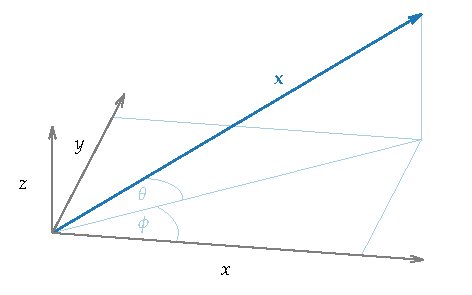
\includegraphics{fig1_05/fig1_05}
    \caption{Coordinate system used in this thesis. The vector $\vec{x}$ can also
    be described by its length, its azimuth angle $\phi$, and its elevation
    $\theta$.
    \reproduce{\GITHUB/fig1_05}}
    \label{fig:coordinate_system}
\end{figure}
%
\paragraph{Coordinate system}
Figure\,\ref{fig:coordinate_system} shows the coordinate system that is used in
the following chapters. A vector $\vec{x}$ can be described by its position
$(x,y,z)$ in space or by its length, azimuth angle $\phi \in [0,2\PI[$,
and elevation $\theta \in \left[-\frac{\PI}{2},\frac{\PI}{2}\right]$.
The azimuth is measured counterclockwise and elevation is positive
for positive $z$-values.


%----%----%----%----%----%----%----%----%----%----%----%----%----%----%----%----
\paragraph{Fourier transformation}
Let $s$ be an absolute integrable function, $t,\omega$ real numbers, then the
temporal Fourier transform is defined as\autocite{Bracewell2000}
%
\begin{equation}
    S(\omega) = \FT{s(t)} = \int^{\infty}_{-\infty} s(t) \E^{-\I\omega t}
    \; \df{t}
    \qp
    \label{eq:ft}
\end{equation}

In the same way the inverse temporal Fourier transform is defined as
%
\begin{equation}
    s(t) = \IFT{S(\omega)} = \frac{1}{2\pi} \int^{\infty}_{-\infty} S(\omega)
    e^{i\omega t} \; d\omega
    \qp
    \label{eq:ift}
\end{equation}
